
%%%%%%%%%%%%%%%%%%%%%%%%%%%%%%%%%%%%%%%%%%%%%%%%%%%%%%%%%%%%%%%%%%%%%
%% This is a (brief) model paper using the achemso class
%% The document class accepts keyval options, which should include
%% the target journal and optionally the manuscript type.
%%%%%%%%%%%%%%%%%%%%%%%%%%%%%%%%%%%%%%%%%%%%%%%%%%%%%%%%%%%%%%%%%%%%%
\documentclass[journal=apchd5,manuscript=article]{achemso}

%%%%%%%%%%%%%%%%%%%%%%%%%%%%%%%%%%%%%%%%%%%%%%%%%%%%%%%%%%%%%%%%%%%%%
%% Place any additional packages needed here.  Only include packages
%% which are essential, to avoid problems later. Do NOT use any
%% packages which require e-TeX (for example etoolbox): the e-TeX
%% extensions are not currently available on the ACS conversion
%% servers.
%%%%%%%%%%%%%%%%%%%%%%%%%%%%%%%%%%%%%%%%%%%%%%%%%%%%%%%%%%%%%%%%%%%%%
\usepackage[version=3]{mhchem} % Formula subscripts using \ce{}
\usepackage[T1]{fontenc}       % Use modern font encodings
\usepackage{graphicx}
\usepackage{amsmath}
\usepackage{xcolor}
\usepackage{wrapfig}
%%%%%%%%%%%%%%%%%%%%%%%%%%%%%%%%%%%%%%%%%%%%%%%%%%%%%%%%%%%%%%%%%%%%%
%% If issues arise when submitting your manuscript, you may want to
%% un-comment the next line.  This provides information on the
%% version of every file you have used.
%%%%%%%%%%%%%%%%%%%%%%%%%%%%%%%%%%%%%%%%%%%%%%%%%%%%%%%%%%%%%%%%%%%%%
%%\listfiles

%%%%%%%%%%%%%%%%%%%%%%%%%%%%%%%%%%%%%%%%%%%%%%%%%%%%%%%%%%%%%%%%%%%%%
%% Place any additional macros here.  Please use \newcommand* where
%% possible, and avoid layout-changing macros (which are not used
%% when typesetting).
%%%%%%%%%%%%%%%%%%%%%%%%%%%%%%%%%%%%%%%%%%%%%%%%%%%%%%%%%%%%%%%%%%%%%
\newcommand*\mycommand[1]{\texttt{\emph{#1}}}

%%%%%%%%%%%%%%%%%%%%%%%%%%%%%%%%%%%%%%%%%%%%%%%%%%%%%%%%%%%%%%%%%%%%%
%% Meta-data block
%% ---------------
%% Each author should be given as a separate \author command.
%%
%% Corresponding authors should have an e-mail given after the author
%% name as an \email command. Phone and fax numbers can be given
%% using \phone and \fax, respectively; this information is optional.
%%
%% The affiliation of authors is given after the authors; each
%% \affiliation command applies to all preceding authors not already
%% assigned an affiliation.
%%
%% The affiliation takes an option argument for the short name.  This
%% will typically be something like "University of Somewhere".
%%
%% The \altaffiliation macro should be used for new address, etc.
%% On the other hand, \alsoaffiliation is used on a per author basis
%% when authors are associated with multiple institutions.
%%%%%%%%%%%%%%%%%%%%%%%%%%%%%%%%%%%%%%%%%%%%%%%%%%%%%%%%%%%%%%%%%%%%%
\author{Nicholas P. Montoni}
\author{Steven C. Quillin}
\author{Charles Cherqui}
\author{David J. Masiello}
\affiliation[Department of Chemistry, University of Washington]
{Department of Chemistry, University of Washington, Seattle, WA 98195}
\email{masiello@chem.washington.edu}

%%%%%%%%%%%%%%%%%%%%%%%%%%%%%%%%%%%%%%%%%%%%%%%%%%%%%%%%%%%%%%%%%%%%%
%% The document title should be given as usual. Some journals require
%% a running title from the author: this should be supplied as an
%% optional argument to \title.
%%%%%%%%%%%%%%%%%%%%%%%%%%%%%%%%%%%%%%%%%%%%%%%%%%%%%%%%%%%%%%%%%%%%%
\title[]
{Tunable Spectral Ordering of Magnetic Plasmons}
%%%%%%%%%%%%%%%%%%%%%%%%%%%%%%%%%%%%%%%%%%%%%%%%%%%%%%%%%%%%%%%%%%%%%
%% Some journals require a list of abbreviations or keywords to be
%% supplied. These should be set up here, and will be printed after
%% the title and author information, if needed.
%%%%%%%%%%%%%%%%%%%%%%%%%%%%%%%%%%%%%%%%%%%%%%%%%%%%%%%%%%%%%%%%%%%%%
\abbreviations{MNP, LSPR, EELS}
\keywords{plasmon, hybridization, magnetic, retardation}

%%%%%%%%%%%%%%%%%%%%%%%%%%%%%%%%%%%%%%%%%%%%%%%%%%%%%%%%%%%%%%%%%%%%%
%% The manuscript does not need to include \maketitle, which is
%% executed automatically.
%%%%%%%%%%%%%%%%%%%%%%%%%%%%%%%%%%%%%%%%%%%%%%%%%%%%%%%%%%%%%%%%%%%%%
\begin{document}

%%%%%%%%%%%%%%%%%%%%%%%%%%%%%%%%%%%%%%%%%%%%%%%%%%%%%%%%%%%%%%%%%%%%%
%% The "tocentry" environment can be used to create an entry for the
%% graphical table of contents. It is given here as some journals
%% require that it is printed as part of the abstract page. It will
%% be automatically moved as appropriate.
%%%%%%%%%%%%%%%%%%%%%%%%%%%%%%%%%%%%%%%%%%%%%%%%%%%%%%%%%%%%%%%%%%%%%
\begin{tocentry}
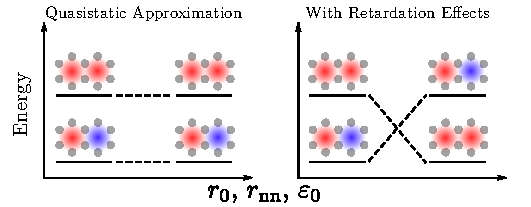
\includegraphics{toc_graphic_2.pdf}

\end{tocentry}

%%%%%%%%%%%%%%%%%%%%%%%%%%%%%%%%%%%%%%%%%%%%%%%%%%%%%%%%%%%%%%%%%%%%%
%% The abstract environment will automatically gobble the contents
%% if an abstract is not used by the target journal.
%%%%%%%%%%%%%%%%%%%%%%%%%%%%%%%%%%%%%%%%%%%%%%%%%%%%%%%%%%%%%%%%%%%%%
\begin{abstract}
Ring-like assemblies of metal nanoparticles that exhibit magnetic resonances, called magnetic plasmon oligomers, have been of recent interest as negative-index metamaterials and light-harvesting devices. For these reasons, it is imperative to understand the properties of such systems on the single- to few-oligomer scale. We show through theory and simulation that the energy ordering of the magnetic resonances of few-oligomer systems depends on size, scale, and environment in ways that purely electric plasmons do not. The dynamic ordering of the eigenmodes of magnetic systems is due entirely to retardation effects and can be understood by inspecting the intermediate- and far-field contributions which are excluded in the quasistatic approximation. This work highlights the versatility and tunability of magnetic plasmon oligomers, elucidating a previously unexplored physical phenomenon and suggesting future applications of magnetic plasmons in highly sensitive detection methods. 
\end{abstract}

%%%%%%%%%%%%%%%%%%%%%%%%%%%%%%%%%%%%%%%%%%%%%%%%%%%%%%%%%%%%%%%%%%%%%
%% Start the main part of the manuscript here.
%%%%%%%%%%%%%%%%%%%%%%%%%%%%%%%%%%%%%%%%%%%%%%%%%%%%%%%%%%%%%%%%%%%%%
\section{Introduction}
Metal nanoparticles (MNPs) support collective resonances of their conduction electrons at optical frequencies. These localized surface plasmon resonances (LSPRs) can interact with each other in assemblies to produce hybridized resonances, much like the hybridization of atomic orbitals in molecules\cite{Lucas1976,ARAVIND1981,Xu1995,Mischenko1995}. When these MNPs are arranged in rings, the single LSPRs can give rise to a collective mode that produces an oscillating magnetic dipole in the center of the ring\cite{Alu2006,Alu2008,Liu2011,Nord2006,Cherqui2014,Cherqui2016}. Such systems are known as magnetic plasmon oligomers and have been of intense focus due to their potential applications in sensing\cite{Zia2010trans,Noginova2008trans,Wang:13,Fan2015,Wei2015,Shvets2012,Altug2012bio,Nord2011fano}, lensing\cite{Fang2005,Valentine2008}, cloaking\cite{Shalaev2008}, and information processing\cite{Zhang2006,NordHal2011,NordHal2012}. In Cherqui's 2014 work on magnetic plasmons, a quasistatic, electric dipole tight-binding model was used to describe the magnetic systems\cite{Cherqui2014}; we adapt this model to expand on the results of that work. Cherqui's model considered only the electric near-field of the single-particle plasmons and only incorporated nearest-neighbor interactions. As a result, while it accurately predicted the magnetic eigenmodes, it inaccurately described the energy ordering predicted by full-wave simulation. An explanation was needed to determine why the tight-binding model would predict different energy-ordering.

In a recent paper, Engheta \textit{et al}. state that magnetic systems are well-understood on the single oligomer scale and the nearly infinite scale\cite{Engheta2017}. Furthermore, the dependence of magnetic properties on individual nanoparticle geometry and the relative size of the constituent oligomers has also been determined\cite{Cherqui2016}. However, the properties of few-oligomer systems have not been fully explored. Here we show that to fully understand the properties of magnetic oligomers on the few-oligomer scale, the simple tight-binding model described above must be extended to include both the fully-retarded electric fields and all inter-particle interactions. We show this through three explorations of oligomer properties: system size, dielectric constant of the environment, and inter-particle spacing, and we confirm our results using full-wave simulations\cite{Hohenester2012}.

It is well-known that as MNPs and aggregates become larger, the quasistatic approximation breaks down. There has been much work done to elucidate the effects of retardation on large MNPs\cite{Abajo2008,Gu2010}, dimers\cite{vonPlessen2007,Rechbacher2003,Kottman2001}, and extended chains and 2-D arrays of particles\cite{Schatz2003,Royer2005,Chumanov2010,Pinchuk2016}. Magnetic oligomers composed of two or more rings of particles have the potential to be hundreds of nanometers to microns across, justifying the need to consider retardation effects in determining their optical properties. In order to incorporate retardation effects into quasistatic plasmon hybridization theory, we begin by mapping the dipole plasmon of each MNP onto a set of harmonic oscillators, and allow them to couple through their electric fields according to the following Hamiltonian\cite{Cherqui2014}:

\begin{equation}
H = \sum_{i}^{n}\frac{\textbf{P}_{i}^{2}}{2m_{\textrm{sp},i}} + \frac{1}{2}m_{\textrm{sp},i}\omega_{\textrm{sp},i}^2\textbf{X}_{i}^{2} - e^2\sum_{i>j}\textbf{X}_i\cdot\boldsymbol{\Lambda}_{ij}\cdot\textbf{X}_j,\label{elec_hammy_1}
\end{equation}

\noindent where $\textbf{P}_i$ are the momenta conjugate to the plasmon coordinates $\textbf{X}_{i}$, $\omega_{\textrm{sp},i}$ are the individual LSPR frequencies of each oscillator, $m_{\textrm{sp},i}$ are the LSPR effective masses and $\boldsymbol{\Lambda}_{ij}$ is the fully retarded dipole-dipole relay tensor (expanded below)\cite{jackson_classical_1999}. To make this Hamiltonian more manageable, it is nondimensionalized using $\textbf{Q}_i = \left(m_{\textrm{sp}}\omega_{\textrm{sp}}/\hbar\right)^{\frac{1}{2}}\textbf{X}_i$ and $\boldsymbol{\Pi}_i = \textbf{P}_i/\sqrt{\hbar m_{\textrm{sp}}\omega_{\textrm{sp}}}$. Substituting into Equation~\ref{elec_hammy_1} and expanding $\boldsymbol{\Lambda}_{ij}$, we get:

\begin{equation}
\begin{aligned}
H = 
\frac{\hbar\omega_{sp}}{2}\sum_{i}^{n}[\boldsymbol{\Pi}_i^2 + \textbf{Q}_i^2] - \frac{\hbar\omega_{sp}}{\varepsilon_b}\sum_{i>j}\{g_{ij}^{\textrm{NF}}\left[3(\textbf{Q}_i\cdot\hat{\textbf{n}}_{ij})(\hat{\textbf{n}}_{ij}\cdot\textbf{Q}_j) - \textbf{Q}_i\cdot\textbf{Q}_j\right] \\
+ g_{ij}^{\textrm{IF}}\left[3(\textbf{Q}_i\cdot\hat{\textbf{n}}_{ij})(\hat{\textbf{n}}_{ij}\cdot\textbf{Q}_j) -\textbf{Q}_i\cdot\textbf{Q}_j\right] \\ 
- g_{ij}^{\textrm{FF}}\left[(\textbf{Q}_i\cdot\hat{\textbf{n}}_{ij})(\hat{\textbf{n}}_{ij}\cdot\textbf{Q}_j) -\textbf{Q}_i\cdot\textbf{Q}_j\right]\},\label{elec_hammy_2}
\end{aligned}
\end{equation}

In this Hamiltonian we introduce the near, intermediate, and far-field coupling terms: $g_{ij}^{\textrm{NF}} = \frac{\alpha_{sp}'}{r_{ij}^3}\cos\left(k r_{ij}\right)$, $g_{ij}^{\textrm{IF}} = \frac{\alpha_{sp}'k}{r_{ij}^2}\sin\left(k r_{ij}\right)$, and $g_{ij}^{\textrm{FF}} = \frac{\alpha_{sp}'k^2}{r_{ij}}\cos\left(k r_{ij}\right)$, respectively, with wavenumber $k = \sqrt{\varepsilon_b}\frac{\omega}{c}$ and $\omega$ is the frequency of each collective mode. Additionally, $r_{ij}$ is the distance between the ith and jth LSPRs and $\hat{\textbf{n}}_{ij}$ is the unit vector connecting two LSPRs. We further incorporate retardation effects by considering the lattice dispersion in the polarizability $\alpha_{sp}' = \left(\alpha_{sp}^{-1} - i\frac{2}{3}k^3\right)^{-1}$ with $\alpha_{sp} = r_0^3\frac{3}{\varepsilon_{\infty}-2\varepsilon_b}$. Including these terms, we have incorporated all retardation effects associated with point dipoles\cite{Purcell1973,Draine1993}.

It should be noted that this Hamiltonian, when diagonalized, results in a transcendental equation whose solutions, the eigenvalues $\omega$, are functions of themselves. In order to fully solve this problem, we make a first guess of $\omega$ for a particular mode of interest and iteratively compute the eigenvalues. Using the eigenvalue associated with the mode of interest, the Hamiltonian is diagonalized to convergence. The process is repeated for each mode of interest.

\section{Results and Discussion}

In this work, we model silver nanoparticles using a Drude model with $\omega_p = 9.1$ eV, $\varepsilon_{\infty} = 3.77$, and $\gamma = 0.003$ eV. Note that we have greatly reduced the damping constant in order to better resolve the magnetic modes in the simulations. The oligomer unit cell is a six-member ring, with silver nanoparticles located at the vertices of a regular hexagon. We explore and manipulate three magnetic oligomer systems: a twomer, a linear threemer, and a triangular threemer. The number of rings in a magnetic system corresponds to the number of magnetic modes in the system\cite{Cherqui2014}. The twomer supports an in-phase mode (North-North, or NN) and an out-of-phase mode (North-South, or NS). The linear threemer supports an all in-phase mode (All-North, or AN), a minimally out-of-phase mode (North-South, or NS), and a maximally out-of-phase mode (North-South-North, or NSN). The triangular threemer supports an all in-phase mode (All-North, or AN) and two degenerate out-of-phase modes (North-South, or NS). These modes and their relative magnetic fields are depicted as insets in Figures~\ref{magmodes},~\ref{interaction_strength},~\ref{dielectric}, and~\ref{spacing}. In each exploration, the particles have radius $r_0$ and nearest-neighbor spacing $r_{\textrm{nn}}$. In the first set of model calculations, we compare to full-wave simulations to verify that the model accurately captures the properties of the systems, but beyond that we cease comparison to simulation in order to focus on the predictive power of the model. The first calculations, depicted in Figure~\ref{magmodes} show how the magnetic modes of the twomer and threemers are impacted by the overall scale of the system. In these calculations, the nearest neighbor distances are held at $r_{\textrm{nn}} = 3 \times r_0$ while $r_0$ varies from 1 nm to 30 nm.

\begin{figure}
\centering
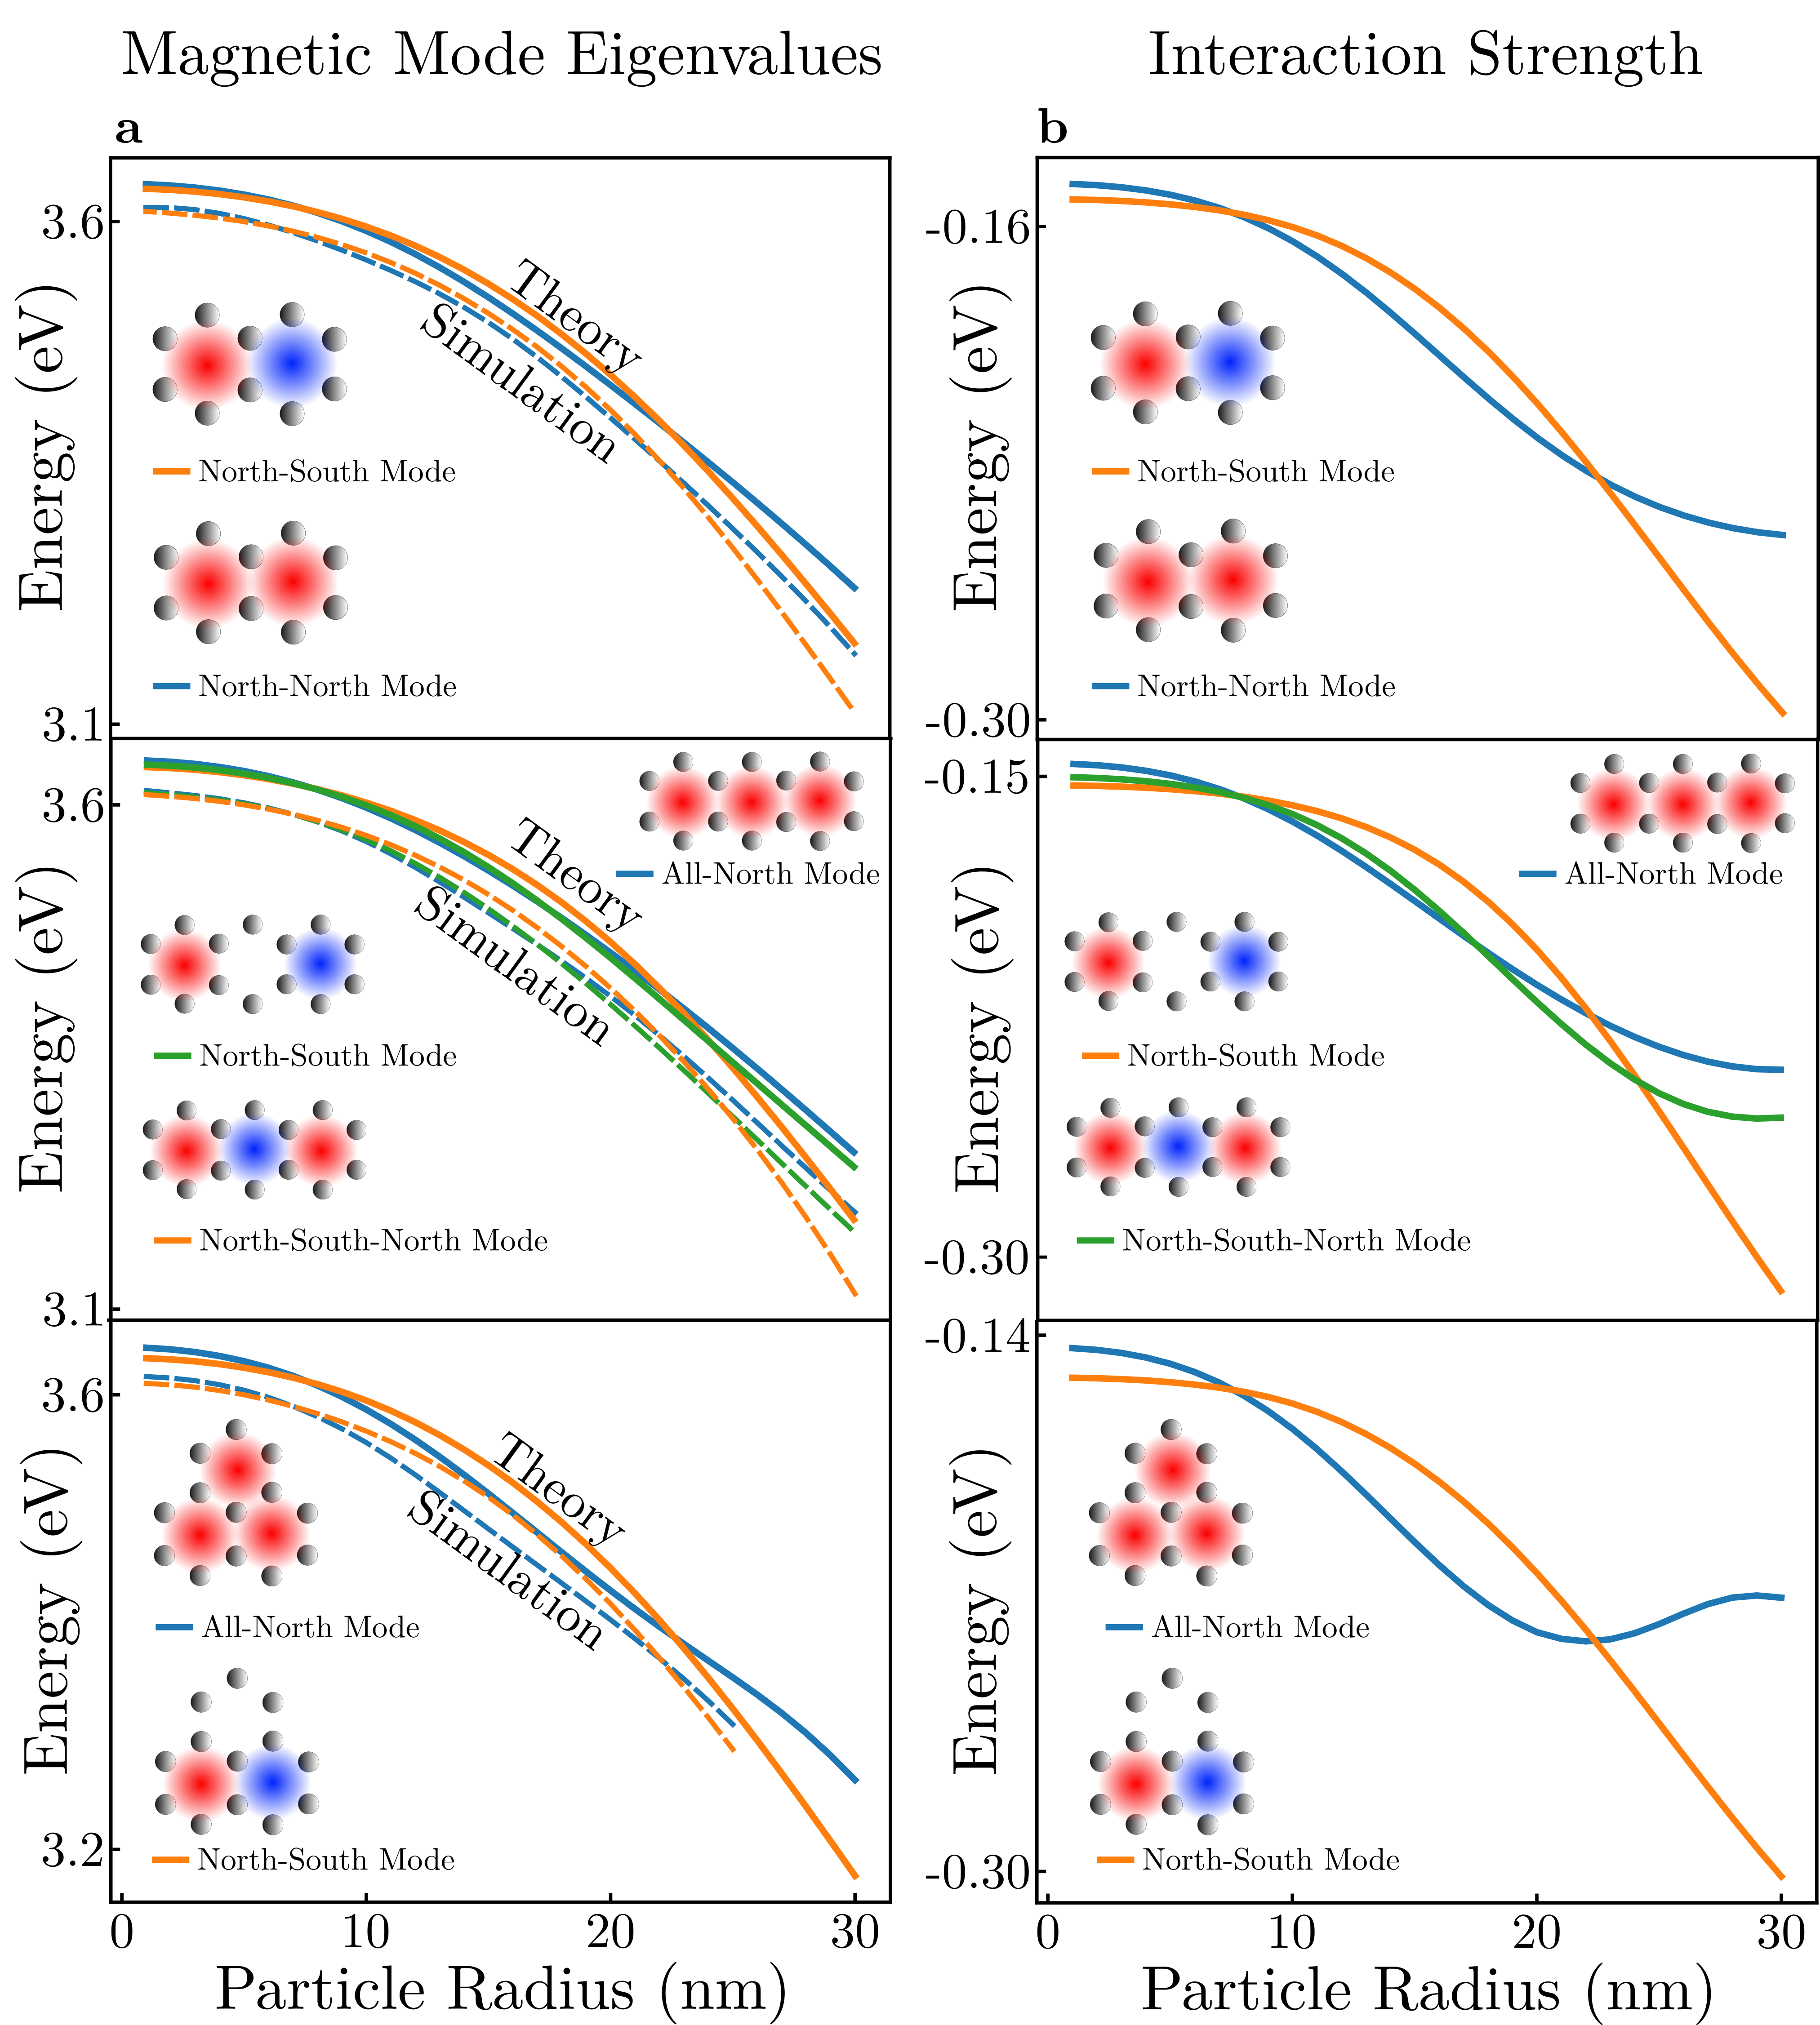
\includegraphics{magnetic_mode_eigenvalues_and_interactions.pdf}
\caption{Magnetic mode eigenvalues (column a), predicted and simulated, and interaction strengths (column b) for the magnetic twomer (first row), linear threemer (second row), and triangular threemer (third row). All of the magnetic modes range from 3.1 eV to 3.6 eV. In each system, the magnetic modes exhibit multiple crossings, showing that the eigenspectrum of these magnetic systems depends on their scale. The model consistently overestimates the eigenvalues by 0.05 eV, and consistently underestimates the crossing points by less than a nanometer. To further emphasize the impact of scale, we have plotted the total interaction strength of each eigenmode, \textit{i.e.} the sum of each eigenvector's dot product with the electric field of all of the other dipoles. This calculation reaffirms the scale-dependence and predicts the same mode crossings as both the eigenvalue calculation and the simulations.}
\label{magmodes}
\end{figure}

In Figure~\ref{magmodes}a, the magnetic mode eigenvalues are computed for each system. The solid lines depict model calculations, and the dashed lines depict simulated results. Interestingly, the magnetic modes exhibit a dynamic energy ordering, switching order twice as a function of scale. It is presumable that they continue to flip at larger and larger sizes. This is confirmed by simulations, with the model overestimating the eigenvalues by about 0.05 eV and underestimating the crossing points by under a nanometer. These small errors are consistent across all three systems. Figure~\ref{magmodes}b displays the computed interaction strength for each eigenmode produced by the tight-binding model,

\begin{equation}
\begin{aligned}
U_{\textrm{int}} = -\sum_{i>j}\textbf{p}_{i}\cdot\boldsymbol{\Lambda}_{ij}\cdot\textbf{p}_{j}
\label{interactionenergy}
\end{aligned}
\end{equation}

\noindent where $\textbf{p}_{i}$ is an eigenvector and $\boldsymbol{\Lambda}_{ij}$ is the dipole relay tensor connecting all of the electric dipoles. This calculation serves as a further confirmation of the mode-switching, as the interaction strengths follow the eigenvalues.

\begin{figure}
\centering
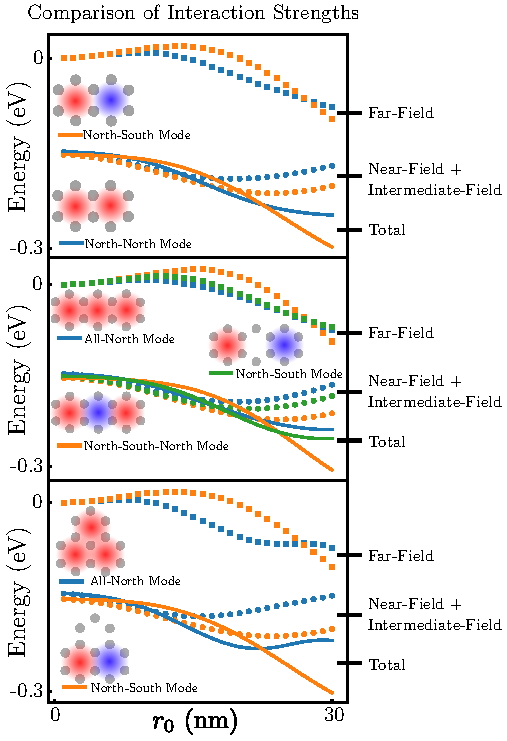
\includegraphics{interaction_strength.pdf}
\caption{Interactions strengths for the magnetic modes of the twomer (first row), linear threemer (second row), and triangular threemer (third row). We plot the total interaction strength between the electric plasmons (solid line), the near-field and intermediate-field interaction strength summed (circles), and the far-field interaction strength (squares) as a function of scaling. The near- and intermediate- fields do not exhibit any crossings and diverge with greater scaling. The far-field terms exhibit one crossing. The interplay of far-field with near- and intermediate-field interactions causes mode-switching in magnetic systems.}
\label{interactions}
\end{figure}

To gain a more complete understanding of this mode-switchings, we compute the total interaction strength for the electric plasmons of each magnetic mode and we break that calculation into its near-, intermediate-, and far-field components. Figure~\ref{interactions} shows that the near- and intermediate-field terms contribute a total shift of the interaction strength, the far-field term alone contributes to the mode switching. This can be seen in the dipole relay tensors for the near- and intermediate-field,

\begin{equation}
\begin{aligned}
\boldsymbol{\Lambda}_{ij}^{\textrm{NF,IF}} \propto 3\hat{\textbf{n}}_{ij}\hat{\textbf{n}}_{ij} -\textbf{1}
\label{lambda_NFIF}
\end{aligned}
\end{equation}

\noindent and the far-field,

\begin{equation}
\begin{aligned}
\boldsymbol{\Lambda}_{ij}^{\textrm{FF}} \propto \textbf{1}-\hat{\textbf{n}}_{ij}\hat{\textbf{n}}_{ij}
\label{lambda_FF}
\end{aligned}
\end{equation}

\noindent where \textbf{1} is the unit dyad. Equations~\ref{lambda_NFIF} and ~\ref{lambda_FF} differ by a factor of 3 on the unit vector term and an overall factor of -1. For this reason, collinear and anticollinear interact more strongly in the near- and intermediate-fields. However, linearly oriented dipoles do not interact through the far-field at all and only parallel and antiparallel dipoles contribute to this term. [\textbf{should I cite the JPCC Steve wrote? Lots about ordering and arrangements of dipoles...}] The factor of -1 difference between Equations~\ref{lambda_NFIF} and ~\ref{lambda_FF} further implies that parallel and anti-parallel arrangements of dipoles will contribute interaction energies of opposite sign. The distance-dependence of each field term for different orientations of dipoles is further outlined in Figure~\ref{dimers}. The opposition of signs, as well as the crossing in the far-field interaction term, explain the phenomenon of mode-switching in magnetic oligomers.

\begin{figure}
\centering
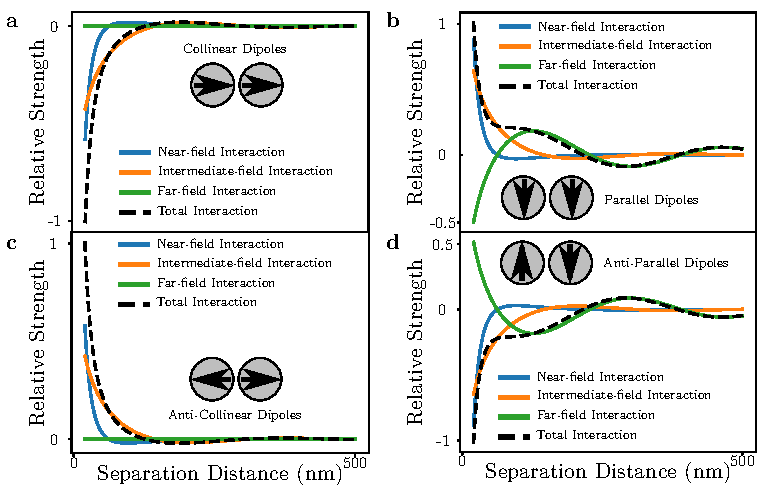
\includegraphics{dimer_interaction.pdf}
\caption{Relative interaction strengths for the four possible dipole arrangements of a nanoparticle dimer: collinear (a), parallel (b), anti-collinear (c), and anti-parallel (d). Plotted are the near-field (blue), intermediate-field (orange), far-field (green), and total (black, dashed) interaction strengths for each set of dipoles as a function of dipole-dipole distance. Interestingly, and stemming from the form of the dipole relay tensor, the far-field interaction term is zero for both pairs of linear dipoles. From these plots, it can be seen that the favorability of a specific dipole arrangement depends on the separation between the dipoles. This can be seen in the fact that each part of the field depends differently on the separation, and each field term contains an oscillating term. At short length scales, the interaction is dominated by the near-field. However, as the distance increases, the interaction is dominated by the intermediate field (a and c) or the far-field (b and d). As a result, there are separation distances at which normally unfavorable arrangements become favorable. Since magnetic oligomers can be described through pairwise interactions of electric dipoles, it follows that the eigenvalues must also change order as different arrangements of electric dipoles become more and less favorable.}
\label{dimers}
\end{figure}

We have convinced ourselves that 1) the quasistatic, nearest-neighbors tight-binding model does not contain enough information to agree with fully retarded electrodynamics simulations, 2) those same simulations conform to the results from an updated tight-binding model that incorporates retardation effects and all-particle interactions and 3) the unexpected mode switching exhibited by these magnetic systems is due to the interplay of the three parts of the fully reatrded electric field. Most notably, without the inclusion of the far-field term and all inter-particle interactions, no mode-switching is observed. With a working model and a basic physical understanding of these three systems, we now perform a series of computations to look at its tunable properties. In the previous section, the scale of the systems was changed. However, this would be impossible to manipulate in a laboratory. We focus on properties with experimental analogues, namely, the dielectric constant of the embedding medium and the nearest-neighbor spacing between nanoparticles.


\begin{figure}
\centering
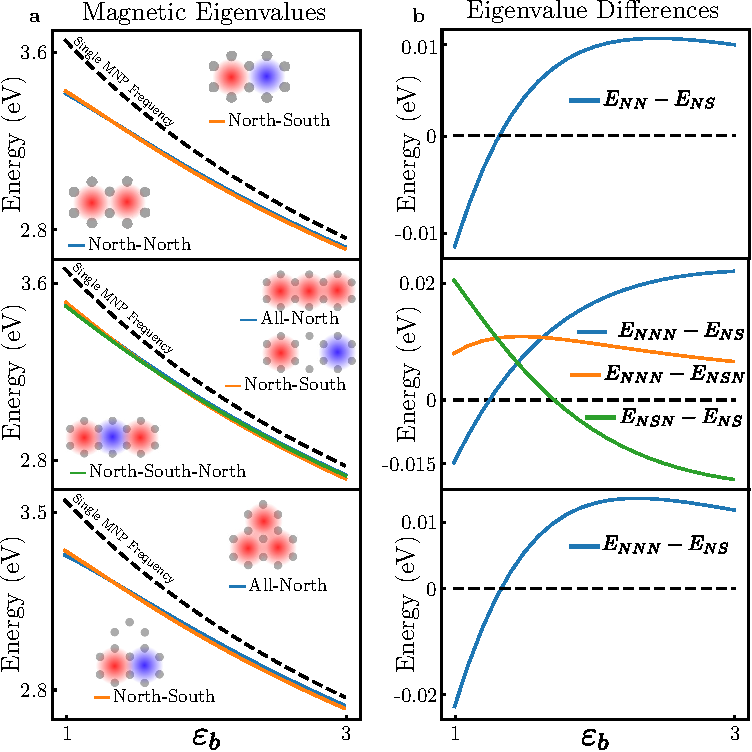
\includegraphics{dielectric_study.pdf}
\caption{Magnetic mode eigenvalues (column a) for the twomer (first row), linear threemer (second row), and triangular threemer (third row) with particle sizes of 20 nm and magnetic mode eigenvalue differences (column b) as a function of the dielectric constant of an embedding medium. As the dielectric constant is increased from 1 to 3, the magnetic mode splitting approaches zero and the overall energy decreases. At very high dielectric values, the magnetic mode eigenvalues converge to the single particle resonance frequency. This is the result of the dielectric constant reducing the inter-particle interactions. It is also important to note that between $\varepsilon_b = 1$ and $\varepsilon_b = 1.5$, the magnetic mode differences vary sharply, either becoming much more positive or much more negative. This is indicative of mode-switching that is difficult to see in the eigenvalue plots. The increasing dielectric constant has a similar effect to increasing the scale of the system, as it recovers the same energy ordering for $r_0 > 20$ nm.}
\label{dielectric}
\end{figure}

In order to justify the next set of model calculations, we refer to research on flowing liquid crystal over MNP aggregates and, in real-time, adjusting the refractive index of the MNP environment, influencing the resonance frequencies of the system\cite{odom_lasing}. We apply this concept to our tight-binding model to determine if this has any implications on the properties of magnetic oligomers. What we find is that, as expected, increasing the real-valued dielectric constant of the background decreases the resonance frequency of the collective modes. Furthermore, the embedding medium influences the energy-ordering of the eigenvalues. Results of one of our explorations are summarized in Figure~\ref{dielectric}. As the dielectric constant of the medium increases, the eigenmodes collapse onto each other, and eventually converge with the single-particle frequency. Because the modes collapse so quickly and appear to overlap at all values of $\varepsilon_b$, Figure~\ref{dielectric}b displays the difference in energy between all of the eigenmodes of each system. The values of $\varepsilon_b$ where the differences cross zero signify mode-crossing. 
From these two observations we conclude that increasing the dielectric constant of the embedding medium weakens the overall inter-particle interactions. However, this occurs differently for each of the parts of the interaction. All of the field terms contain similar $k$-dependence through $\alpha_{\textrm{sp}}'$ and the trigonometric terms. Focusing on the different $k$-dependence in each of the coupling contants (~\ref{elec_hammy_2}) reveals the infuence of the dielectric constant on the electric field. $g_{ij}^\textrm{NF}$ contains no other $k$-dependence, so the near-field contribution is reduced by one factor of $\varepsilon_b$.  $g_{ij}^\textrm{IF}$ is linear in $k$, so it is reduced by a factor of $\sqrt{\varepsilon_b}$. Lastly,  $g_{ij}^\textrm{FF}$ is quadratic in $k$, so all $\varepsilon_b$-dependence is removed, besides that dependence previously mentioned. At higher values of the dielectric constant the far-field term dominates, much like the way particles that are far apart interact primarily through their far-fields (Figure~\ref{dimers}b and d). In other words, embedding magnetic systems in some dielectric medium causes them to act as though they are larger, effectively increasing their scale. This insight provides an experimental route to directly choosing the energy-ordering of magnetic modes, but the reduced splitting between modes might make such an experiment infeasible.

\begin{figure}
\centering
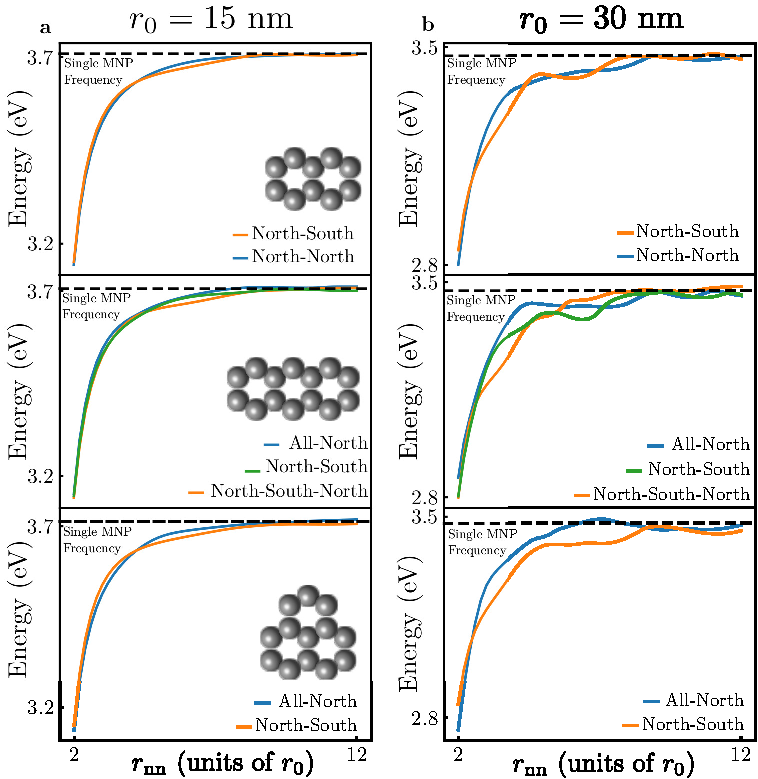
\includegraphics{spacing_study.pdf}
\caption{Magnetic mode eigenvalues for the twomer (first row), linear threemer (second row), and triangular threemer (third row) with particle sizes of 15 nm (column a) and 30 nm (column b) as a function of nearest neighbor particle separation in units of radii. As the separation distance increases, the magnetic mode eigenvalues converge to and oscillate about the single particle frequency, exhibiting multiple crossings. As in Equation~\ref{elec_hammy_2}, the interaction strength decays with increasing separation and oscillates due to its dependence on trigonometric functions.}
\label{spacing}
\end{figure}

Another topic of great interest is tuning the size and shape of a plasmonic aggregate using various polymers\cite{Ginger2017} or DNA\cite{DanLuo2009,NaLiu2017}. Here, we implement the idea of continuously distorting the nearest-neighbor spacing, from touching to tens of radii apart. We present data for particle radii of 15 nm and 30 nm in Figure~\ref{spacing}a and b, respectively. The results of these model calculations are reminiscent of the results in Figure~\ref{dimers} in that the eigenmodes oscillate about each other as the particles move farther apart. In addition, similarly to Figure~\ref{dielectric}, at very large distances the eigenvalues converge to the single LSPR frequency, exhibiting small amplitude oscillations. This is indicative of the coupling falling very near to zero. It is clear that this method, as opposed to the method of tuning the dielectric constant of the background, offers a much greater degree of tunability. Designing a system in which the inter-particle spacing could be varied in discrete steps would lead to the ability to directly choose the resonance frequency of a specific magnetic mode. Furthermore, being able to directly detect the frequency of the magnetic mode optically could turn such magnetic systems into thermometers, pH probes, or detectors of any environmental factor that would change the size of the embedding polymer.

%%%%%%%%%%%%%%%%%%%%%%%%%%%%%%%%%%%%%%%%%%%%%%%%%%%%%%%%%%%%%%%%%%%%%%%%%%
%% CONCLUSION. I DON'T THINK ACS NANO HAS A DISTINCT CONCLUSION SECTION %%
%%%%%%%%%%%%%%%%%%%%%%%%%%%%%%%%%%%%%%%%%%%%%%%%%%%%%%%%%%%%%%%%%%%%%%%%%%

\section{Conclusion}
We have shown that magnetic systems on the few-oligomer scale exhibit tunable resonances with dynamic spectral ordering. This unique property is due to the interplay of near-, intermediate-, and far-field interactions and the variation of those interactions with size, distance, and the dielectric constant of the environment. However, we stress that the systems studied in this work were chosen due to their theoretical simplicity. In simulated and experimental spectroscopies, these eigenmodes would overlap and be nearly indistinguishable. It has been shown that oligomers whose constituents are rod-like, elongated, or generally degeneracy-breaking have sharper, more isolated magnetic resonances\cite{Cherqui2016}. To this end, future studies will involve these geometries to determine if they have the same eigenmode-switching properties and tunability. With this groundwork on the properties of small oligomers, there is now an incentive and an avenue to expanding the concepts presented here to larger aggregates, as well as a need to confirm the predictions made here with experiments. The ability of the researcher to decide the resonance frequency of a particular eigenmode opens the door to the ability to dynamically and actively determine system properties.

%%%%%%%%%%%%%%%%%%%%%%%%%%%%%%%%%%%%%%%%%%%%%%%%%%%%%%%%%%%%%%%%%%%%%
%% The ``Acknowledgment'' section can be given in all manuscript
%% classes.  This should be given within the ``acknowledgment''
%% environment, which will make the correct section or running title.
%%%%%%%%%%%%%%%%%%%%%%%%%%%%%%%%%%%%%%%%%%%%%%%%%%%%%%%%%%%%%%%%%%%%%
\begin{acknowledgement}
CEI, NSF, DOE?, Niket, some other people, probably, HPC.
\end{acknowledgement}

%%%%%%%%%%%%%%%%%%%%%%%%%%%%%%%%%%%%%%%%%%%%%%%%%%%%%%%%%%%%%%%%%%%%%
%% The appropriate \bibliography command should be placed here.
%% Notice that the class file automatically sets \bibliographystyle
%% and also names the section correctly.
%%%%%%%%%%%%%%%%%%%%%%%%%%%%%%%%%%%%%%%%%%%%%%%%%%%%%%%%%%%%%%%%%%%%%
\bibliography{references}
\end{document}
